% !TeX program = pdflatex
\documentclass[tikz,border=8pt]{standalone}
\usepackage{tikz}
\definecolor{FigureBlue}{HTML}{2563EB}
\begin{document}
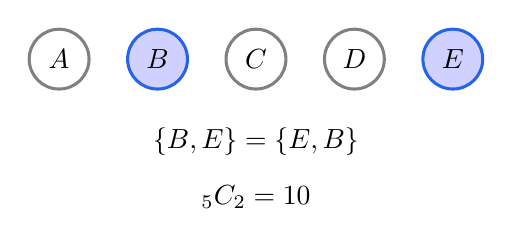
\begin{tikzpicture}
  \foreach \i/\lab in {0/A,2/C,3/D}{\draw[fill=white,draw=gray,line width=1.1pt] (1.25*\i,0) circle (.38);\node at (1.25*\i,0) {$\lab$};}
  \foreach \i/\lab in {1/B,4/E}{\draw[fill=blue!18,draw=FigureBlue,line width=1.1pt] (1.25*\i,0) circle (.38);\node at (1.25*\i,0) {$\lab$};}
  \node at (2.5,-1.05) {$\{B,E\}=\{E,B\}$}; \node at (2.5,-1.75) {${}_{5}C_{2}=10$};
\end{tikzpicture}
\end{document}
